\documentclass{article}
\usepackage{arxiv}

\usepackage[utf8]{inputenc}
\usepackage[english, russian]{babel}
\usepackage[T1]{fontenc}
\usepackage{url}
\usepackage{booktabs}
\usepackage{amsfonts}
\usepackage{nicefrac}
\usepackage{microtype}
\usepackage{lipsum}
\usepackage{graphicx}
\usepackage{natbib}
\usepackage{doi}
\usepackage{amsmath}



\title{Post Training Quantization. Flexible continuous modification for SOTA post training quantization methods to make them lossless.}

\author{ David S.~Hippocampus\thanks{Use footnote for providing further
		information about author (webpage, alternative
		address)---\emph{not} for acknowledging funding agencies.} \\
	Department of Computer Science\\
	Cranberry-Lemon University\\
	Pittsburgh, PA 15213 \\
	\texttt{hippo@cs.cranberry-lemon.edu} \\
	%% examples of more authors
	\And
	Elias D.~Striatum \\
	Department of Electrical Engineering\\
	Mount-Sheikh University\\
	Santa Narimana, Levand \\
	\texttt{stariate@ee.mount-sheikh.edu} \\
	%% \AND
	%% Coauthor \\
	%% Affiliation \\
	%% Address \\
	%% \texttt{email} \\
	%% \And
	%% Coauthor \\
	%% Affiliation \\
	%% Address \\
	%% \texttt{email} \\
	%% \And
	%% Coauthor \\
	%% Affiliation \\
	%% Address \\
	%% \texttt{email} \\
}
\date{}

\renewcommand{\shorttitle}{\textit{arXiv} Template}

%%% Add PDF metadata to help others organize their library
%%% Once the PDF is generated, you can check the metadata with
%%% $ pdfinfo template.pdf
\hypersetup{
pdftitle={A template for the arxiv style},
pdfsubject={q-bio.NC, q-bio.QM},
pdfauthor={David S.~Hippocampus, Elias D.~Striatum},
pdfkeywords={First keyword, Second keyword, More},
}

\begin{document}
\maketitle

\begin{abstract}
Neural network quantization gives the opportunity to inference large models on resource constrained devices. Post training quantization methods have became popular, as they are simple to use. They don't require whole model retraining and use only small calibration set to calculate quantization parameters. However, these methods show significant accuracy decrease on low-bit quantization. There are methods that allow to increase the accuracy of model by increasing its computational complexity. In this paper, we propose a continuous modification for these methods,  and find a reasonable compromise between computational complexity and quantization efficiency.
\end{abstract}


\keywords{First keyword \and Second keyword \and More}

\section{Introduction}
Deep Neural Networks(DNN) are applicable to wide range of tasks nowadays. Despite showing the great performance on these tasks, state-of-the-art models require high computational resources. There is a need to run large models on power-limited devices such as smartphones. Many different methods were proposed for model compression. In this paper, we concentrate on quantization method.

The quantization is a process of  mapping real numbers to the low-precision discrete values. There are two main types of quantization methods: quantization aware training(QAT) and post training quantization(PTQ). Quantization aware training shows great results, however, it requires the whole model retraining. Hence, this method is not applicable in some real-life cases, as if training data is not available or computational resources are limited. Unlike QAT, post training quantization usually uses only an unlabeled calibration set for setting up quantization. Current post quantization methods are not such efficient as quantization aware training. However, post training quantization is a promising technique and therefore should be explored further.

The goal of post training quantization is to find optimal quantization parameters having only small set of data. The main problem of this technique is that quantization errors of layers can be amplified by deeper layers.  Quantization errors can accumulate layer by layer and lead to accuracy degradation. Quantization accuracy degradation is explored in the \citep{loss-aware-quantization} article, which explaines why  low-bit post-training quantization is a quite challenging task.  

Most of post training quantization methods quantize model parameters and data by minimizing the error between quantized and the original model layers outputs. The recent post quantization techniques  \citep{adaquant, BreQ} made a progress towards low-bit post training quantization, considering previous layers errors during quantization. However, these methods leave model structure 
without changes and don't consider improving accuracy of quantized model by complicating its structure.  

In this work, we study ways to improve quantized model accuracy by making model more complex. Paper  \citep{multiple_points}  uses the idea of approximating model weights as a sum of low-precision values. Our paper suggests a modification to this method.  There are two main goals of this work. Firstly, we would like to propose a method to make post training quantization lossless. This is relevant to situations when computational device support only low bit data types. Second approach of this paper is to find a trade-off between model complexity and quantization bits, allowing to compress model for resource constrained devices.  








\section{Problem statement section}
\label{sec:headings}
In this article, we use uniform quantization. Given value to quantize $v$ , the maximum and minimum quantization value $Q_{max}$ and $Q_{min}$ and quantization step size $\Delta$, quantizer computes integer representation of a data $\bar{v}$:
$$
 \bar{v} =
\begin{cases}
    -Q_{min}, \text{if} \frac{v}{\Delta} \leq -Q_{min}\\
    \lfloor\frac{v}{\Delta}\rceil, \text{if} \frac{v}{\Delta} \in [-Q_{min}, Q_{max}]\\
    Q_{max}, \text{if} \frac{v}{\Delta} \geq Q_{max}\\
\end{cases}.
$$
To get representation of the same scale, $\bar{v}$ is multiplied by $\Delta$:
$$
\hat{v} = \bar{v} * \Delta.
$$
Let's suppose that that we calculate the quantization of each parameter $W$ $K_W$ times, denote $K = (K_{W_1}, ... K_{W_N})$, where $W_1, ..., W_N$ - model parameters.
Also let $\Delta$ be a vector containing quantization parameters for all weights and data. \\

The goal of our work is to quantize model M without significant performance degradation. We will achieve this by making  outputs of $Q(M, \Delta, K)$ similar to the outputs of M, where $Q(M, \Delta, K)$ is a denotion for quantized model M with parameters $K,\ \Delta$. For comparing models outputs, we will use some loss function $L(M1, M2, dataset)$. \\

Let's denote model M complexity as $P(M)$.

Then, we want to minimize $L(M, Q(M, \Delta, K), dataset)$  for given model M, calibration dataset $dataset$ and some complexity limit $P_0$:

$argmin_{K, \Delta} \{L(M, Q(M, \Delta, K), dataset),  P(M, K, \Delta) \leq P_0\}$

\subsection{Headings: second level}
\lipsum[5]
\begin{equation}
	\xi _{ij}(t)=P(x_{t}=i,x_{t+1}=j|y,v,w;\theta)= {\frac {\alpha _{i}(t)a^{w_t}_{ij}\beta _{j}(t+1)b^{v_{t+1}}_{j}(y_{t+1})}{\sum _{i=1}^{N} \sum _{j=1}^{N} \alpha _{i}(t)a^{w_t}_{ij}\beta _{j}(t+1)b^{v_{t+1}}_{j}(y_{t+1})}}
\end{equation}

\subsubsection{Headings: third level}
\lipsum[6]

\paragraph{Paragraph}
\lipsum[7]



\section{Examples of citations, figures, tables, references}
\label{sec:others}

\subsection{Citations}
Citations use \verb+natbib+. The documentation may be found at
\begin{center}
	\url{http://mirrors.ctan.org/macros/latex/contrib/natbib/natnotes.pdf}
\end{center}

Here is an example usage of the two main commands (\verb+citet+ and \verb+citep+): Some people thought a thing \citep{kour2014real, hadash2018estimate} but other people thought something else \citep{kour2014fast}. Many people have speculated that if we knew exactly why \citet{kour2014fast} thought this\dots

\subsection{Figures}
\lipsum[10]
See Figure \ref{fig:fig1}. Here is how you add footnotes. \footnote{Sample of the first footnote.}
\lipsum[11]

\begin{figure}
	\centering
	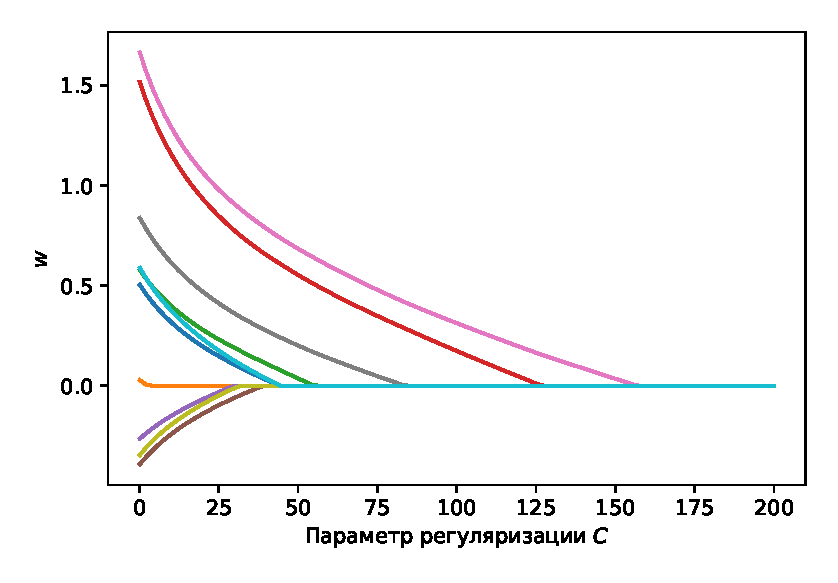
\includegraphics[width=0.5\textwidth]{../figures/log_reg_cs_exp.eps}
	\caption{Sample figure caption.}
	\label{fig:fig1}
\end{figure}

\subsection{Tables}
See awesome Table~\ref{tab:table}.

The documentation for \verb+booktabs+ (`Publication quality tables in LaTeX') is available from:
\begin{center}
	\url{https://www.ctan.org/pkg/booktabs}
\end{center}


\begin{table}
	\caption{Sample table title}
	\centering
	\begin{tabular}{lll}
		\toprule
		\multicolumn{2}{c}{Part}                   \\
		\cmidrule(r){1-2}
		Name     & Description     & Size ($\mu$m) \\
		\midrule
		Dendrite & Input terminal  & $\sim$100     \\
		Axon     & Output terminal & $\sim$10      \\
		Soma     & Cell body       & up to $10^6$  \\
		\bottomrule
	\end{tabular}
	\label{tab:table}
\end{table}

\subsection{Lists}
\begin{itemize}
	\item Lorem ipsum dolor sit amet
	\item consectetur adipiscing elit.
	\item Aliquam dignissim blandit est, in dictum tortor gravida eget. In ac rutrum magna.
\end{itemize}


\bibliographystyle{unsrtnat}
\bibliography{references}

\end{document}
